\documentclass{book}
\usepackage[a4paper,top=2.5cm,bottom=2.5cm,left=2.5cm,right=2.5cm]{geometry}
\usepackage{makeidx}
\usepackage{natbib}
\usepackage{graphicx}
\usepackage{multicol}
\usepackage{float}
\usepackage{listings}
\usepackage{color}
\usepackage{ifthen}
\usepackage[table]{xcolor}
\usepackage{textcomp}
\usepackage{alltt}
\usepackage{ifpdf}
\ifpdf
\usepackage[pdftex,
            pagebackref=true,
            colorlinks=true,
            linkcolor=blue,
            unicode
           ]{hyperref}
\else
\usepackage[ps2pdf,
            pagebackref=true,
            colorlinks=true,
            linkcolor=blue,
            unicode
           ]{hyperref}
\usepackage{pspicture}
\fi
\usepackage[utf8]{inputenc}
\usepackage{polski}
\usepackage[T1]{fontenc}

\usepackage{mathptmx}
\usepackage[scaled=.90]{helvet}
\usepackage{courier}
\usepackage{sectsty}
\usepackage{amssymb}
\usepackage[titles]{tocloft}
\usepackage{doxygen}
\lstset{language=C++,inputencoding=utf8,basicstyle=\footnotesize,breaklines=true,breakatwhitespace=true,tabsize=4,numbers=left }
\makeindex
\setcounter{tocdepth}{3}
\renewcommand{\footrulewidth}{0.4pt}
\renewcommand{\familydefault}{\sfdefault}
\hfuzz=15pt
\setlength{\emergencystretch}{15pt}
\hbadness=750
\tolerance=750
\begin{document}
\hypersetup{pageanchor=false,citecolor=blue}
\begin{titlepage}
\vspace*{7cm}
\begin{center}
{\Large My Project }\\
\vspace*{1cm}
{\large Wygenerowano przez Doxygen 1.8.3.1}\\
\vspace*{0.5cm}
{\small Śr, 21 maj 2014 19:49:02}\\
\end{center}
\end{titlepage}
\clearemptydoublepage
\pagenumbering{roman}
\tableofcontents
\clearemptydoublepage
\pagenumbering{arabic}
\hypersetup{pageanchor=true,citecolor=blue}
\chapter{Dokumentacja zadania P\-A\-M\-S\-I L\-A\-B 1}
\label{index}\hypertarget{index}{}\begin{DoxyAuthor}{Autor}
Karolina Morawska 
\end{DoxyAuthor}
\begin{DoxyDate}{Data}
16.\-03.\-2014 
\end{DoxyDate}
\begin{DoxyVersion}{Wersja}
0.\-2 
\end{DoxyVersion}

\chapter{Indeks klas}
\section{Lista klas}
Tutaj znajdują się klasy, struktury, unie i interfejsy wraz z ich krótkimi opisami\-:\begin{DoxyCompactList}
\item\contentsline{section}{\hyperlink{class_n_o_d_e}{N\-O\-D\-E} \\*Modeluje pojęcie \hyperlink{class_n_o_d_e}{N\-O\-D\-E} ,czyli wezel. Klasa modeluje pojęcie node . Jej atrybutem są pola zawierające wskaźnik na lewy ,prawy węzeł i wartość }{\pageref{class_n_o_d_e}}{}
\item\contentsline{section}{\hyperlink{class_para}{Para} \\*Modeluje pojęcie \hyperlink{class_para}{Para}. Klasa modeluje pojęcie para . Jej atrybutem są pola zawierające klucz i wartość }{\pageref{class_para}}{}
\item\contentsline{section}{\hyperlink{classper}{per$<$ K, W $>$} \\*Modeluje pojęcie per. Klasa modeluje pojęcie per(para) . Jej atrybutem są pola zawierające klucz i wartość }{\pageref{classper}}{}
\item\contentsline{section}{\hyperlink{class_tablicaas}{Tablicaas$<$ K, W $>$} \\*Modeluje pojęcie \hyperlink{class_tablicaas}{Tablicaas}. Klasa modeluje pojęcie Tablica asocjacyjna . Jej atrybutem są pola zawierające klucz i wartość }{\pageref{class_tablicaas}}{}
\item\contentsline{section}{\hyperlink{class_tree}{Tree} \\*Modeluje pojęcie \hyperlink{class_para}{Para}. Klasa modeluje pojęcie para . Jej atrybutem jest pole zawierajace root(korzen) }{\pageref{class_tree}}{}
\end{DoxyCompactList}

\chapter{Indeks plików}
\section{Lista plików}
Tutaj znajduje się lista wszystkich plików z ich krótkimi opisami\-:\begin{DoxyCompactList}
\item\contentsline{section}{\hyperlink{czas_8hh}{czas.\-hh} }{\pageref{czas_8hh}}{}
\item\contentsline{section}{\hyperlink{dzialania_8cpp}{dzialania.\-cpp} }{\pageref{dzialania_8cpp}}{}
\item\contentsline{section}{\hyperlink{dzialania_8hh}{dzialania.\-hh} }{\pageref{dzialania_8hh}}{}
\item\contentsline{section}{\hyperlink{kolejka_8hh}{kolejka.\-hh} }{\pageref{kolejka_8hh}}{}
\item\contentsline{section}{\hyperlink{main_8cpp}{main.\-cpp} }{\pageref{main_8cpp}}{}
\item\contentsline{section}{\hyperlink{stos_8hh}{stos.\-hh} }{\pageref{stos_8hh}}{}
\item\contentsline{section}{\hyperlink{stos2_8hh}{stos2.\-hh} }{\pageref{stos2_8hh}}{}
\item\contentsline{section}{\hyperlink{stoslista_8hh}{stoslista.\-hh} }{\pageref{stoslista_8hh}}{}
\item\contentsline{section}{\hyperlink{tablica_8cpp}{tablica.\-cpp} }{\pageref{tablica_8cpp}}{}
\item\contentsline{section}{\hyperlink{tablica_8hh}{tablica.\-hh} }{\pageref{tablica_8hh}}{}
\end{DoxyCompactList}

\chapter{Dokumentacja klas}
\hypertarget{class_dzialania}{\section{Dokumentacja klasy Dzialania}
\label{class_dzialania}\index{Dzialania@{Dzialania}}
}


Deklaracja klasy \hyperlink{class_dzialania}{Dzialania}.  




{\ttfamily \#include $<$dzialania.\-hh$>$}

\subsection*{Metody publiczne}
\begin{DoxyCompactItemize}
\item 
bool \hyperlink{class_dzialania_a4d1a1b41a0f2f76d4c16ad20f77b7cfa}{wczytajplik} (char $\ast$nazwapl)
\item 
bool \hyperlink{class_dzialania_af059b80e034854eb1ae878d6b636fff6}{porownaj} (char $\ast$nazwapl)
\item 
double \hyperlink{class_dzialania_a8c13fb89281d74f9dd8dd22f43bffbb9}{liczczas} (int iloscpowtorzen)
\item 
int \hyperlink{class_dzialania_a177e69d16b8280aae1d658adb67a8fbc}{rozmiartab} ()
\end{DoxyCompactItemize}


\subsection{Opis szczegółowy}
Deklaracja klasy \hyperlink{class_dzialania}{Dzialania}. 

Klasa \hyperlink{class_dzialania}{Dzialania} posiada pola oraz funkcje potrzebne do wykonywania dzialan na tablicach . 

Definicja w linii 11 pliku dzialania.\-hh.



\subsection{Dokumentacja funkcji składowych}
\hypertarget{class_dzialania_a8c13fb89281d74f9dd8dd22f43bffbb9}{\index{Dzialania@{Dzialania}!liczczas@{liczczas}}
\index{liczczas@{liczczas}!Dzialania@{Dzialania}}
\subsubsection[{liczczas}]{\setlength{\rightskip}{0pt plus 5cm}double Dzialania\-::liczczas (
\begin{DoxyParamCaption}
\item[{int}]{iloscpowtorzen}
\end{DoxyParamCaption}
)}}\label{class_dzialania_a8c13fb89281d74f9dd8dd22f43bffbb9}
Funkcja mierzy czas dzialania algorytmu.

Argumenty i najwazniejsze pola funkcji -\/iloscpowtorzen -\/zmienna zawierajaca ile powtorzen ma wykonywac program. 

Definicja w linii 80 pliku dzialania.\-cpp.

\hypertarget{class_dzialania_af059b80e034854eb1ae878d6b636fff6}{\index{Dzialania@{Dzialania}!porownaj@{porownaj}}
\index{porownaj@{porownaj}!Dzialania@{Dzialania}}
\subsubsection[{porownaj}]{\setlength{\rightskip}{0pt plus 5cm}bool Dzialania\-::porownaj (
\begin{DoxyParamCaption}
\item[{char $\ast$}]{nazwapl}
\end{DoxyParamCaption}
)}}\label{class_dzialania_af059b80e034854eb1ae878d6b636fff6}
Funkcja porownuje dwa pliki \-: plik wejsciowy i sprawdzajacy , informuje o porawnosci wykonywanego $\ast$ dzialania.

Argumenty i najwazniejsze pola funkcji -\/nazwapl zmienna typu char zawierajaca nazwe pliku 

Definicja w linii 49 pliku dzialania.\-cpp.

\hypertarget{class_dzialania_a177e69d16b8280aae1d658adb67a8fbc}{\index{Dzialania@{Dzialania}!rozmiartab@{rozmiartab}}
\index{rozmiartab@{rozmiartab}!Dzialania@{Dzialania}}
\subsubsection[{rozmiartab}]{\setlength{\rightskip}{0pt plus 5cm}int Dzialania\-::rozmiartab (
\begin{DoxyParamCaption}
{}
\end{DoxyParamCaption}
)\hspace{0.3cm}{\ttfamily [inline]}}}\label{class_dzialania_a177e69d16b8280aae1d658adb67a8fbc}
Funkcja pomocnicza zwraca rozmiar tablicy . 

Definicja w linii 34 pliku dzialania.\-hh.

\hypertarget{class_dzialania_a4d1a1b41a0f2f76d4c16ad20f77b7cfa}{\index{Dzialania@{Dzialania}!wczytajplik@{wczytajplik}}
\index{wczytajplik@{wczytajplik}!Dzialania@{Dzialania}}
\subsubsection[{wczytajplik}]{\setlength{\rightskip}{0pt plus 5cm}bool Dzialania\-::wczytajplik (
\begin{DoxyParamCaption}
\item[{char $\ast$}]{nazwapl}
\end{DoxyParamCaption}
)}}\label{class_dzialania_a4d1a1b41a0f2f76d4c16ad20f77b7cfa}
Funkcja wczytujaca plik i sprawdzajaca porawnosc wykonania funkcji.

Argumenty i najwazniejsze pola funkcji -\/nazwapl zmienna typu char zawierajaca nazwe pliku 

Definicja w linii 24 pliku dzialania.\-cpp.



Dokumentacja dla tej klasy została wygenerowana z plików\-:\begin{DoxyCompactItemize}
\item 
/home/karolina/\-Pulpit/pamsi/prj/inc/\hyperlink{dzialania_8hh}{dzialania.\-hh}\item 
/home/karolina/\-Pulpit/pamsi/prj/src/\hyperlink{dzialania_8cpp}{dzialania.\-cpp}\end{DoxyCompactItemize}

\hypertarget{class_tablica}{\section{Dokumentacja klasy Tablica}
\label{class_tablica}\index{Tablica@{Tablica}}
}


Deklaracja klasy \hyperlink{class_tablica}{Tablica}.  




{\ttfamily \#include $<$tablica.\-hh$>$}

\subsection*{Metody publiczne}
\begin{DoxyCompactItemize}
\item 
void \hyperlink{class_tablica_a4f69d95776f0ea1454a87bb72562713b}{zamienelementy} (int i, int j)
\begin{DoxyCompactList}\small\item\em Funkcja sluzaca do zamiany elementow. \end{DoxyCompactList}\item 
void \hyperlink{class_tablica_ad4d99dc2ca07689167d703ba24a4dab2}{dodajelement} (int element)
\begin{DoxyCompactList}\small\item\em Funkcja dodaje element na tablice.\-Wykorzystuje funkcje pomocnicza $\ast$ zmiana rozmiaru. \end{DoxyCompactList}\item 
void \hyperlink{class_tablica_ae63b8d381eb4f6a19cae52241228ae07}{odwrockolejnosc} ()
\begin{DoxyCompactList}\small\item\em Funkcja odwraca kolejnosc w tablicy. \end{DoxyCompactList}\item 
void \hyperlink{class_tablica_ac5b21c0e98c4f5ac5c728b99f092b112}{dodajelementy} (const \hyperlink{class_tablica}{Tablica} \&T1)
\begin{DoxyCompactList}\small\item\em Funkcja laczy ze soba dwie tablice. \end{DoxyCompactList}\item 
\hyperlink{class_tablica_a5f484e7b0478e1ff9b62e894f9d7b28d}{Tablica} ()
\begin{DoxyCompactList}\small\item\em Konstruktor klasy \hyperlink{class_tablica}{Tablica}. \end{DoxyCompactList}\item 
\hyperlink{class_tablica_a6e1e50608ad0f9f9626d0b1fb698b180}{$\sim$\-Tablica} ()
\begin{DoxyCompactList}\small\item\em Destruktor klasy \hyperlink{class_tablica}{Tablica}. \end{DoxyCompactList}\item 
unsigned int \hyperlink{class_tablica_ae95a62ea4245e732b96c110c0fc53532}{rozmiar} () const 
\begin{DoxyCompactList}\small\item\em Funkcja pomocnicza zwraca dlugosc tablicy. \end{DoxyCompactList}\item 
void \hyperlink{class_tablica_a4e743bdbb74647717d63015894dfae8d}{zmianarozmiaru} (unsigned int nowyrozmiar)
\begin{DoxyCompactList}\small\item\em Funkcja pomocnicza sluzaca do zmiany rozmiaru . \end{DoxyCompactList}\item 
int \& \hyperlink{class_tablica_aa73e557bfd1a0283d94b594f159cf6d1}{operator\mbox{[}$\,$\mbox{]}} (const unsigned int b)
\item 
const int \& \hyperlink{class_tablica_a16a2591adbcce8add22be48ff8f1a830}{operator\mbox{[}$\,$\mbox{]}} (const unsigned int b) const 
\item 
\hyperlink{class_tablica}{Tablica} \& \hyperlink{class_tablica_a469a403559ecce37e70c8adc67a0fc0d}{operator+} (const \hyperlink{class_tablica}{Tablica} \&argument) const 
\begin{DoxyCompactList}\small\item\em Przeciazenie operatora dodawania. \end{DoxyCompactList}\item 
\hyperlink{class_tablica}{Tablica} \& \hyperlink{class_tablica_af42a963c962250d20240811a0defd6b4}{operator=} (const \hyperlink{class_tablica}{Tablica} \&argument)
\begin{DoxyCompactList}\small\item\em Przeciazenie operatora przypisywania. \end{DoxyCompactList}\item 
bool \hyperlink{class_tablica_a9416cdb689731ec64d440de10d944549}{operator==} (const \hyperlink{class_tablica}{Tablica} \&argument) const 
\begin{DoxyCompactList}\small\item\em Przeciazenie operatora porownania. \end{DoxyCompactList}\end{DoxyCompactItemize}
\subsection*{Atrybuty prywatne}
\begin{DoxyCompactItemize}
\item 
int $\ast$ \hyperlink{class_tablica_a0b8cd5b5744d8758471455946bc6c8ee}{T}
\begin{DoxyCompactList}\small\item\em Pole przechowujeca wskaznik do tablicy. \end{DoxyCompactList}\item 
unsigned int \hyperlink{class_tablica_ab6ba0fd6c21f6dc5564a8180b2d6bc69}{dlugosctab}
\begin{DoxyCompactList}\small\item\em Pole przechowujace dlugosc tablicy. \end{DoxyCompactList}\end{DoxyCompactItemize}


\subsection{Opis szczegółowy}
Klasa \hyperlink{class_tablica}{Tablica} posiada pola oraz funkcje potrzebne do wykonywania dzialan na tablicach. 

Definicja w linii 13 pliku tablica.\-hh.



\subsection{Dokumentacja konstruktora i destruktora}
\hypertarget{class_tablica_a5f484e7b0478e1ff9b62e894f9d7b28d}{\index{Tablica@{Tablica}!Tablica@{Tablica}}
\index{Tablica@{Tablica}!Tablica@{Tablica}}
\subsubsection[{Tablica}]{\setlength{\rightskip}{0pt plus 5cm}Tablica\-::\-Tablica (
\begin{DoxyParamCaption}
{}
\end{DoxyParamCaption}
)\hspace{0.3cm}{\ttfamily [inline]}}}\label{class_tablica_a5f484e7b0478e1ff9b62e894f9d7b28d}


Definicja w linii 44 pliku tablica.\-hh.



Oto graf wywoływań tej funkcji\-:\nopagebreak
\begin{figure}[H]
\begin{center}
\leavevmode
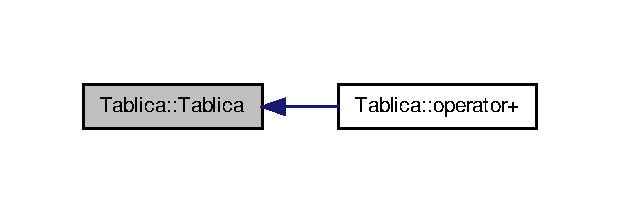
\includegraphics[width=298pt]{class_tablica_a5f484e7b0478e1ff9b62e894f9d7b28d_icgraph}
\end{center}
\end{figure}


\hypertarget{class_tablica_a6e1e50608ad0f9f9626d0b1fb698b180}{\index{Tablica@{Tablica}!$\sim$\-Tablica@{$\sim$\-Tablica}}
\index{$\sim$\-Tablica@{$\sim$\-Tablica}!Tablica@{Tablica}}
\subsubsection[{$\sim$\-Tablica}]{\setlength{\rightskip}{0pt plus 5cm}Tablica\-::$\sim$\-Tablica (
\begin{DoxyParamCaption}
{}
\end{DoxyParamCaption}
)\hspace{0.3cm}{\ttfamily [inline]}}}\label{class_tablica_a6e1e50608ad0f9f9626d0b1fb698b180}


Definicja w linii 48 pliku tablica.\-hh.



\subsection{Dokumentacja funkcji składowych}
\hypertarget{class_tablica_ad4d99dc2ca07689167d703ba24a4dab2}{\index{Tablica@{Tablica}!dodajelement@{dodajelement}}
\index{dodajelement@{dodajelement}!Tablica@{Tablica}}
\subsubsection[{dodajelement}]{\setlength{\rightskip}{0pt plus 5cm}void Tablica\-::dodajelement (
\begin{DoxyParamCaption}
\item[{int}]{element}
\end{DoxyParamCaption}
)}}\label{class_tablica_ad4d99dc2ca07689167d703ba24a4dab2}
Argumenty i najwazniejsze pola funkcji -\/element -\/zmienna ktora zostaje dodana do tablicy 

Definicja w linii 47 pliku tablica.\-cpp.



Oto graf wywołań dla tej funkcji\-:\nopagebreak
\begin{figure}[H]
\begin{center}
\leavevmode
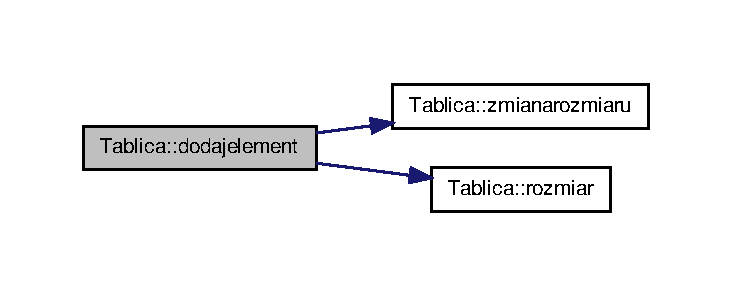
\includegraphics[width=350pt]{class_tablica_ad4d99dc2ca07689167d703ba24a4dab2_cgraph}
\end{center}
\end{figure}


\hypertarget{class_tablica_ac5b21c0e98c4f5ac5c728b99f092b112}{\index{Tablica@{Tablica}!dodajelementy@{dodajelementy}}
\index{dodajelementy@{dodajelementy}!Tablica@{Tablica}}
\subsubsection[{dodajelementy}]{\setlength{\rightskip}{0pt plus 5cm}void Tablica\-::dodajelementy (
\begin{DoxyParamCaption}
\item[{const {\bf Tablica} \&}]{T1}
\end{DoxyParamCaption}
)}}\label{class_tablica_ac5b21c0e98c4f5ac5c728b99f092b112}
Argumenty i najwazniejsze pola funkcji -\/\-T1 -\/tablica ktora powtaje po polaczeniu. 

Definicja w linii 56 pliku tablica.\-cpp.



Oto graf wywołań dla tej funkcji\-:\nopagebreak
\begin{figure}[H]
\begin{center}
\leavevmode
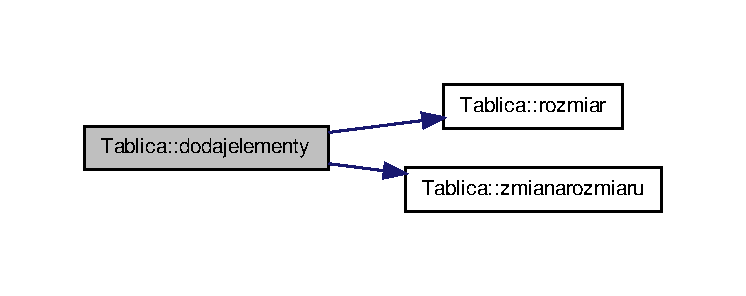
\includegraphics[width=350pt]{class_tablica_ac5b21c0e98c4f5ac5c728b99f092b112_cgraph}
\end{center}
\end{figure}




Oto graf wywoływań tej funkcji\-:\nopagebreak
\begin{figure}[H]
\begin{center}
\leavevmode
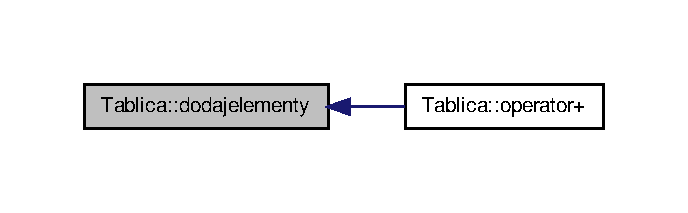
\includegraphics[width=330pt]{class_tablica_ac5b21c0e98c4f5ac5c728b99f092b112_icgraph}
\end{center}
\end{figure}


\hypertarget{class_tablica_ae63b8d381eb4f6a19cae52241228ae07}{\index{Tablica@{Tablica}!odwrockolejnosc@{odwrockolejnosc}}
\index{odwrockolejnosc@{odwrockolejnosc}!Tablica@{Tablica}}
\subsubsection[{odwrockolejnosc}]{\setlength{\rightskip}{0pt plus 5cm}void Tablica\-::odwrockolejnosc (
\begin{DoxyParamCaption}
{}
\end{DoxyParamCaption}
)}}\label{class_tablica_ae63b8d381eb4f6a19cae52241228ae07}
Argumenty i najwazniejsze pola funkcji -\/dlugosctab -\/zmmienna zawierajaca dlugosc tablicy na ktorej wykonywane jest dzialania 

Definicja w linii 25 pliku tablica.\-cpp.



Oto graf wywołań dla tej funkcji\-:\nopagebreak
\begin{figure}[H]
\begin{center}
\leavevmode
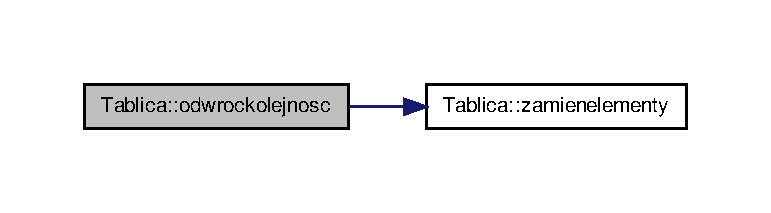
\includegraphics[width=350pt]{class_tablica_ae63b8d381eb4f6a19cae52241228ae07_cgraph}
\end{center}
\end{figure}


\hypertarget{class_tablica_a469a403559ecce37e70c8adc67a0fc0d}{\index{Tablica@{Tablica}!operator+@{operator+}}
\index{operator+@{operator+}!Tablica@{Tablica}}
\subsubsection[{operator+}]{\setlength{\rightskip}{0pt plus 5cm}{\bf Tablica} \& Tablica\-::operator+ (
\begin{DoxyParamCaption}
\item[{const {\bf Tablica} \&}]{argument}
\end{DoxyParamCaption}
) const}}\label{class_tablica_a469a403559ecce37e70c8adc67a0fc0d}
Argumenty i najwazniejsze pola funkcji -\/argument -\/przecciazenie operatora 

Definicja w linii 80 pliku tablica.\-cpp.



Oto graf wywołań dla tej funkcji\-:\nopagebreak
\begin{figure}[H]
\begin{center}
\leavevmode
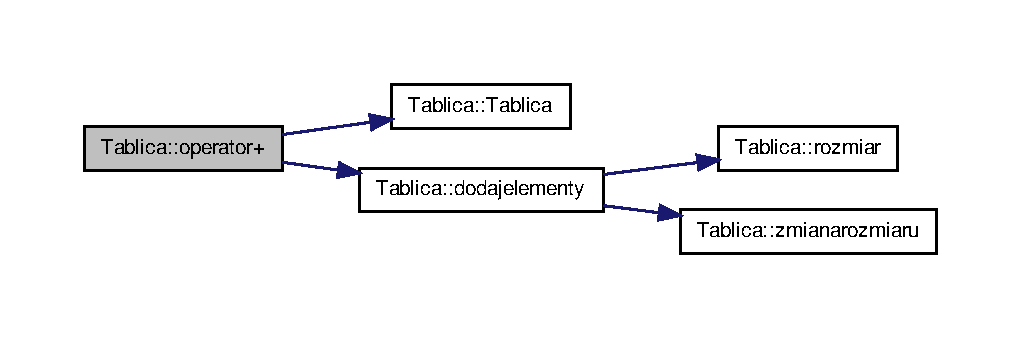
\includegraphics[width=350pt]{class_tablica_a469a403559ecce37e70c8adc67a0fc0d_cgraph}
\end{center}
\end{figure}


\hypertarget{class_tablica_af42a963c962250d20240811a0defd6b4}{\index{Tablica@{Tablica}!operator=@{operator=}}
\index{operator=@{operator=}!Tablica@{Tablica}}
\subsubsection[{operator=}]{\setlength{\rightskip}{0pt plus 5cm}{\bf Tablica} \& Tablica\-::operator= (
\begin{DoxyParamCaption}
\item[{const {\bf Tablica} \&}]{argument}
\end{DoxyParamCaption}
)}}\label{class_tablica_af42a963c962250d20240811a0defd6b4}
Argumenty i najwazniejsze pola funkcji -\/agrument -\/przeciazenie operatora 

Definicja w linii 68 pliku tablica.\-cpp.



Oto graf wywołań dla tej funkcji\-:\nopagebreak
\begin{figure}[H]
\begin{center}
\leavevmode
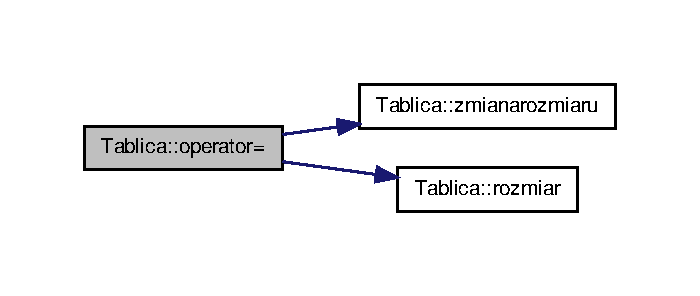
\includegraphics[width=336pt]{class_tablica_af42a963c962250d20240811a0defd6b4_cgraph}
\end{center}
\end{figure}


\hypertarget{class_tablica_a9416cdb689731ec64d440de10d944549}{\index{Tablica@{Tablica}!operator==@{operator==}}
\index{operator==@{operator==}!Tablica@{Tablica}}
\subsubsection[{operator==}]{\setlength{\rightskip}{0pt plus 5cm}bool Tablica\-::operator== (
\begin{DoxyParamCaption}
\item[{const {\bf Tablica} \&}]{argument}
\end{DoxyParamCaption}
) const}}\label{class_tablica_a9416cdb689731ec64d440de10d944549}
Argumenty i najwazniejsze pola funkcji -\/argumenti -\/przeciazenie operatora 

Definicja w linii 93 pliku tablica.\-cpp.



Oto graf wywołań dla tej funkcji\-:\nopagebreak
\begin{figure}[H]
\begin{center}
\leavevmode
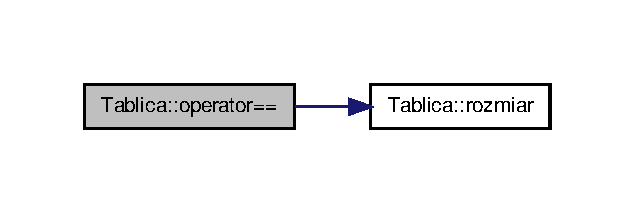
\includegraphics[width=304pt]{class_tablica_a9416cdb689731ec64d440de10d944549_cgraph}
\end{center}
\end{figure}


\hypertarget{class_tablica_aa73e557bfd1a0283d94b594f159cf6d1}{\index{Tablica@{Tablica}!operator\mbox{[}$\,$\mbox{]}@{operator[]}}
\index{operator\mbox{[}$\,$\mbox{]}@{operator[]}!Tablica@{Tablica}}
\subsubsection[{operator[]}]{\setlength{\rightskip}{0pt plus 5cm}int\& Tablica\-::operator\mbox{[}$\,$\mbox{]} (
\begin{DoxyParamCaption}
\item[{const unsigned int}]{b}
\end{DoxyParamCaption}
)\hspace{0.3cm}{\ttfamily [inline]}}}\label{class_tablica_aa73e557bfd1a0283d94b594f159cf6d1}
\textbackslash{} brief Przeciazenie operatora indeksujacego. 

Definicja w linii 60 pliku tablica.\-hh.

\hypertarget{class_tablica_a16a2591adbcce8add22be48ff8f1a830}{\index{Tablica@{Tablica}!operator\mbox{[}$\,$\mbox{]}@{operator[]}}
\index{operator\mbox{[}$\,$\mbox{]}@{operator[]}!Tablica@{Tablica}}
\subsubsection[{operator[]}]{\setlength{\rightskip}{0pt plus 5cm}const int\& Tablica\-::operator\mbox{[}$\,$\mbox{]} (
\begin{DoxyParamCaption}
\item[{const unsigned int}]{b}
\end{DoxyParamCaption}
) const\hspace{0.3cm}{\ttfamily [inline]}}}\label{class_tablica_a16a2591adbcce8add22be48ff8f1a830}


Definicja w linii 61 pliku tablica.\-hh.

\hypertarget{class_tablica_ae95a62ea4245e732b96c110c0fc53532}{\index{Tablica@{Tablica}!rozmiar@{rozmiar}}
\index{rozmiar@{rozmiar}!Tablica@{Tablica}}
\subsubsection[{rozmiar}]{\setlength{\rightskip}{0pt plus 5cm}unsigned int Tablica\-::rozmiar (
\begin{DoxyParamCaption}
{}
\end{DoxyParamCaption}
) const\hspace{0.3cm}{\ttfamily [inline]}}}\label{class_tablica_ae95a62ea4245e732b96c110c0fc53532}


Definicja w linii 52 pliku tablica.\-hh.



Oto graf wywoływań tej funkcji\-:\nopagebreak
\begin{figure}[H]
\begin{center}
\leavevmode
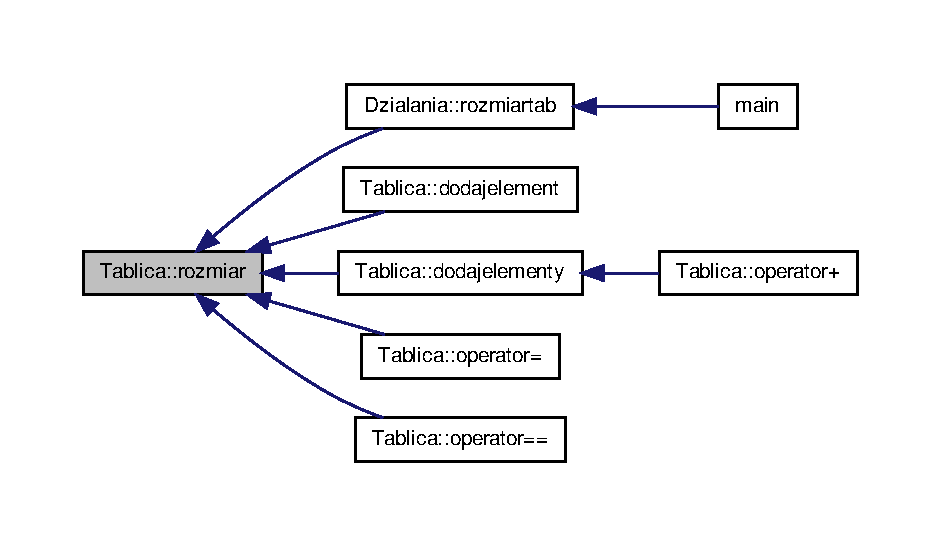
\includegraphics[width=350pt]{class_tablica_ae95a62ea4245e732b96c110c0fc53532_icgraph}
\end{center}
\end{figure}


\hypertarget{class_tablica_a4f69d95776f0ea1454a87bb72562713b}{\index{Tablica@{Tablica}!zamienelementy@{zamienelementy}}
\index{zamienelementy@{zamienelementy}!Tablica@{Tablica}}
\subsubsection[{zamienelementy}]{\setlength{\rightskip}{0pt plus 5cm}void Tablica\-::zamienelementy (
\begin{DoxyParamCaption}
\item[{int}]{i, }
\item[{int}]{j}
\end{DoxyParamCaption}
)}}\label{class_tablica_a4f69d95776f0ea1454a87bb72562713b}
Argumenty i najwazniejsze pola funkcji -\/i, j -\/zmienne oznaczajace elementy w tablicy 

Definicja w linii 12 pliku tablica.\-cpp.



Oto graf wywoływań tej funkcji\-:\nopagebreak
\begin{figure}[H]
\begin{center}
\leavevmode
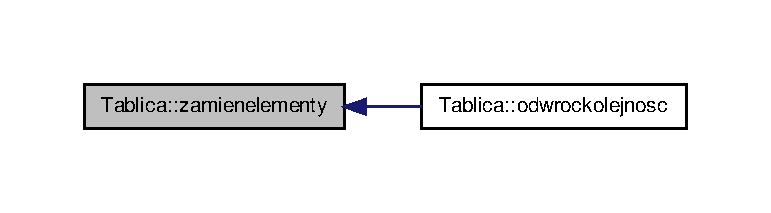
\includegraphics[width=350pt]{class_tablica_a4f69d95776f0ea1454a87bb72562713b_icgraph}
\end{center}
\end{figure}


\hypertarget{class_tablica_a4e743bdbb74647717d63015894dfae8d}{\index{Tablica@{Tablica}!zmianarozmiaru@{zmianarozmiaru}}
\index{zmianarozmiaru@{zmianarozmiaru}!Tablica@{Tablica}}
\subsubsection[{zmianarozmiaru}]{\setlength{\rightskip}{0pt plus 5cm}void Tablica\-::zmianarozmiaru (
\begin{DoxyParamCaption}
\item[{unsigned int}]{nowyrozmiar}
\end{DoxyParamCaption}
)}}\label{class_tablica_a4e743bdbb74647717d63015894dfae8d}
Argumenty i najwazniejsze pola funkcji \begin{DoxyReturn}{Zwraca}
nowyrozmiar -\/\-Rozmiar tablicy po zmianie. 
\end{DoxyReturn}


Definicja w linii 37 pliku tablica.\-cpp.



Oto graf wywoływań tej funkcji\-:\nopagebreak
\begin{figure}[H]
\begin{center}
\leavevmode
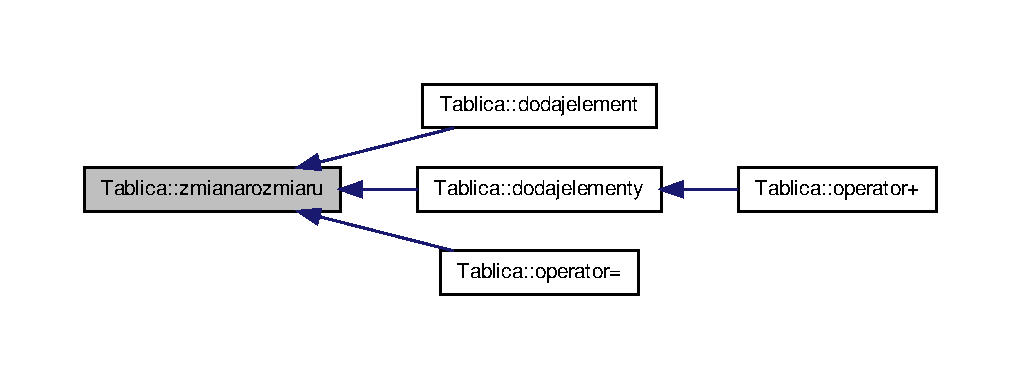
\includegraphics[width=350pt]{class_tablica_a4e743bdbb74647717d63015894dfae8d_icgraph}
\end{center}
\end{figure}




\subsection{Dokumentacja atrybutów składowych}
\hypertarget{class_tablica_ab6ba0fd6c21f6dc5564a8180b2d6bc69}{\index{Tablica@{Tablica}!dlugosctab@{dlugosctab}}
\index{dlugosctab@{dlugosctab}!Tablica@{Tablica}}
\subsubsection[{dlugosctab}]{\setlength{\rightskip}{0pt plus 5cm}unsigned int Tablica\-::dlugosctab\hspace{0.3cm}{\ttfamily [private]}}}\label{class_tablica_ab6ba0fd6c21f6dc5564a8180b2d6bc69}


Definicja w linii 22 pliku tablica.\-hh.

\hypertarget{class_tablica_a0b8cd5b5744d8758471455946bc6c8ee}{\index{Tablica@{Tablica}!T@{T}}
\index{T@{T}!Tablica@{Tablica}}
\subsubsection[{T}]{\setlength{\rightskip}{0pt plus 5cm}int$\ast$ Tablica\-::\-T\hspace{0.3cm}{\ttfamily [private]}}}\label{class_tablica_a0b8cd5b5744d8758471455946bc6c8ee}


Definicja w linii 18 pliku tablica.\-hh.



Dokumentacja dla tej klasy została wygenerowana z plików\-:\begin{DoxyCompactItemize}
\item 
\hyperlink{tablica_8hh}{tablica.\-hh}\item 
\hyperlink{tablica_8cpp}{tablica.\-cpp}\end{DoxyCompactItemize}

\chapter{Dokumentacja plików}
\hypertarget{dzialania_8cpp}{\section{Dokumentacja pliku /home/karolina/\-Pulpit/pamsi/prj/src/dzialania.cpp}
\label{dzialania_8cpp}\index{/home/karolina/\-Pulpit/pamsi/prj/src/dzialania.\-cpp@{/home/karolina/\-Pulpit/pamsi/prj/src/dzialania.\-cpp}}
}
{\ttfamily \#include $<$iostream$>$}\\*
{\ttfamily \#include $<$fstream$>$}\\*
{\ttfamily \#include $<$dzialania.\-hh$>$}\\*
{\ttfamily \#include $<$ctime$>$}\\*
Wykres zależności załączania dla dzialania.\-cpp\-:

\hypertarget{dzialania_8hh}{\section{Dokumentacja pliku /home/karolina/\-Pulpit/pamsi/prj/inc/dzialania.hh}
\label{dzialania_8hh}\index{/home/karolina/\-Pulpit/pamsi/prj/inc/dzialania.\-hh@{/home/karolina/\-Pulpit/pamsi/prj/inc/dzialania.\-hh}}
}
{\ttfamily \#include \char`\"{}tablica.\-hh\char`\"{}}\\*
Wykres zależności załączania dla dzialania.\-hh\-:\nopagebreak
\begin{figure}[H]
\begin{center}
\leavevmode
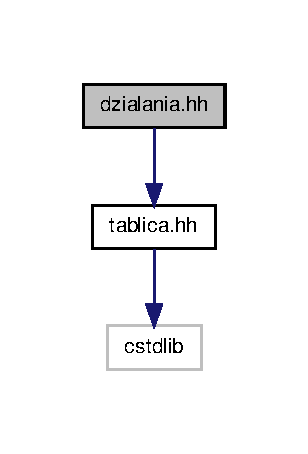
\includegraphics[width=264pt]{dzialania_8hh__incl}
\end{center}
\end{figure}
Ten wykres pokazuje, które pliki bezpośrednio lub pośrednio załączają ten plik\-:\nopagebreak
\begin{figure}[H]
\begin{center}
\leavevmode
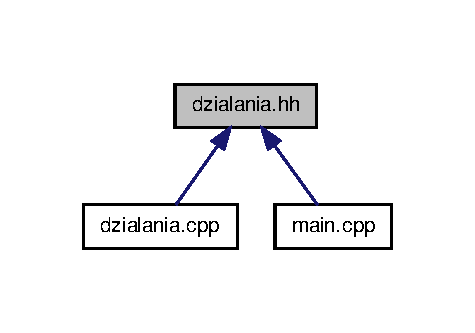
\includegraphics[width=216pt]{dzialania_8hh__dep__incl}
\end{center}
\end{figure}
\subsection*{Komponenty}
\begin{DoxyCompactItemize}
\item 
class \hyperlink{class_dzialania}{Dzialania}
\begin{DoxyCompactList}\small\item\em Deklaracja klasy \hyperlink{class_dzialania}{Dzialania}. \end{DoxyCompactList}\end{DoxyCompactItemize}

\hypertarget{main_8cpp}{\section{Dokumentacja pliku /home/karolina/\-Pulpit/pamsi/prj/src/main.cpp}
\label{main_8cpp}\index{/home/karolina/\-Pulpit/pamsi/prj/src/main.\-cpp@{/home/karolina/\-Pulpit/pamsi/prj/src/main.\-cpp}}
}
{\ttfamily \#include $<$iostream$>$}\\*
{\ttfamily \#include $<$dzialania.\-hh$>$}\\*
{\ttfamily \#include $<$cstdlib$>$}\\*
Wykres zależności załączania dla main.\-cpp\-:
\subsection*{Funkcje}
\begin{DoxyCompactItemize}
\item 
int \hyperlink{main_8cpp_a3c04138a5bfe5d72780bb7e82a18e627}{main} (int argc, char $\ast$$\ast$argv)
\begin{DoxyCompactList}\small\item\em Funkcja main wykonuje algorytm i sprawdza czas dzialania algorytmu. W funkcji main wykonywane sa operacje \-: -\/\-Wczytywanie pliku z danymi wejsciowym -\/\-Dane sa mnozone razy 2 (w tej chwili wlaczany jest stoper) -\/\-Wczytywanie pliku z danymi sprawdzajacymi -\/\-Sprawdzanie zgodnosci -\/\-Stoper zostaje wylaczony i na wyjsciu programu podany zostaje czas dzialania algorytmu. \end{DoxyCompactList}\end{DoxyCompactItemize}


\subsection{Dokumentacja funkcji}
\hypertarget{main_8cpp_a3c04138a5bfe5d72780bb7e82a18e627}{\index{main.\-cpp@{main.\-cpp}!main@{main}}
\index{main@{main}!main.cpp@{main.\-cpp}}
\subsubsection[{main}]{\setlength{\rightskip}{0pt plus 5cm}int main (
\begin{DoxyParamCaption}
\item[{int}]{argc, }
\item[{char $\ast$$\ast$}]{argv}
\end{DoxyParamCaption}
)}}\label{main_8cpp_a3c04138a5bfe5d72780bb7e82a18e627}


Funkcja main wykonuje algorytm i sprawdza czas dzialania algorytmu. W funkcji main wykonywane sa operacje \-: -\/\-Wczytywanie pliku z danymi wejsciowym -\/\-Dane sa mnozone razy 2 (w tej chwili wlaczany jest stoper) -\/\-Wczytywanie pliku z danymi sprawdzajacymi -\/\-Sprawdzanie zgodnosci -\/\-Stoper zostaje wylaczony i na wyjsciu programu podany zostaje czas dzialania algorytmu. 



Definicja w linii 22 pliku main.\-cpp.


\hypertarget{tablica_8cpp}{\section{Dokumentacja pliku tablica.\-cpp}
\label{tablica_8cpp}\index{tablica.\-cpp@{tablica.\-cpp}}
}


Metody klasy \hyperlink{class_tablica}{Tablica}.  


{\ttfamily \#include $<$tablica.\-hh$>$}\\*
{\ttfamily \#include $<$iostream$>$}\\*
Wykres zależności załączania dla tablica.\-cpp\-:\nopagebreak
\begin{figure}[H]
\begin{center}
\leavevmode
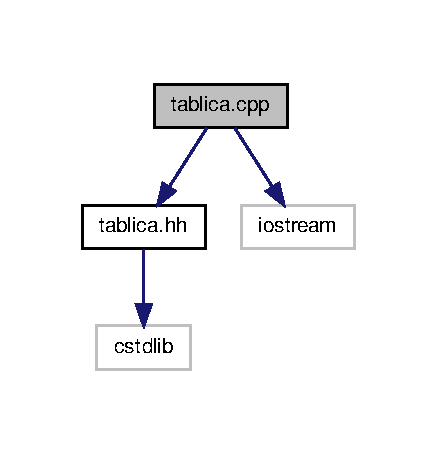
\includegraphics[width=210pt]{tablica_8cpp__incl}
\end{center}
\end{figure}

\hypertarget{tablica_8hh}{\section{Dokumentacja pliku tablica.\-hh}
\label{tablica_8hh}\index{tablica.\-hh@{tablica.\-hh}}
}
{\ttfamily \#include $<$iostream$>$}\\*
{\ttfamily \#include $<$cstdlib$>$}\\*
Wykres zależności załączania dla tablica.\-hh\-:
Ten wykres pokazuje, które pliki bezpośrednio lub pośrednio załączają ten plik\-:
\subsection*{Komponenty}
\begin{DoxyCompactItemize}
\item 
class \hyperlink{class_tablica}{Tablica$<$ Typ $>$}
\begin{DoxyCompactList}\small\item\em Szablon klasy \hyperlink{class_tablica}{Tablica}. \end{DoxyCompactList}\end{DoxyCompactItemize}

\addcontentsline{toc}{part}{Indeks}
\printindex
\end{document}
